\subsubsection{Le gaborium}

\paragraph{Le dispositif}Le gaborium utilise également des \glspl{gabor} comme stimulus. Un écran rempli d'une multitudes de gabors de tailles et d'orientations différentes est montré
au sujet. Tous les distracteurs sont des gabors avec une direction et une vitesse de mouvement constante. La cible est un gabor dont la direction et la vitesse changent constamment.
Dans cette tâche, le sujet doit cliquer sur la cible avec la souris des qu'il l'aperçoit. La cible disparaît alors et une autre cible fait son apparition après un laps de temps
variable. L'œil droit du sujet est traqué à l'aide d'un eye tracker Eyelink. Il doit également appuyer sur la barre espace s'il sent qu'il n'est plus concentré sur la tâche de Gaborium.

\begin{figure}[H]
    \begin{center}
    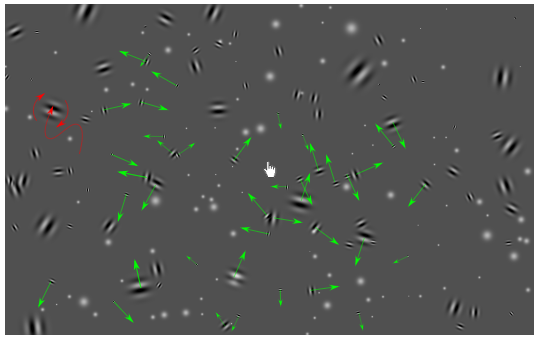
\includegraphics[width=13cm]{gaborium.png}
    \end{center}
    \caption{Gaborium avec les directions de certains gabors affichées}
\label{Gaborium}
\end{figure}

\paragraph{Traitement des données}\textcolor{red}{Il faut traiter les données mais on sait pas comment donc il faut demander à Simon !!!}